	\section{QoS Budget and Priority Collaborative Optimization}
	\label{section_config_opt}

    This section extends the priority optimization algorithm in Section~\ref{section_priority_opt} to solve the joint problem of optimizing priority assignments and QoS options.

    The key observation is that a QoS-configurable task ($\tau^Q_i$) can be treated as a special type of environment-dependent task ($\tau^E_i$): the scheduler is the ``environment'' that decides Qos-configurable tasks' execution time distribution.
    Therefore, we can decompose the joint optimization problem into QoS and priority optimization sub-problems. 
    During the searching of QoS configurations, the incremental optimization can be utilized to co-optimize priority assignments of QoS tasks efficiently. Figure~\ref{fig:overall_workflow} illustrates the overall collaborative optimization algorithm.
    
    \begin{figure*}[htbp]
        \centering
        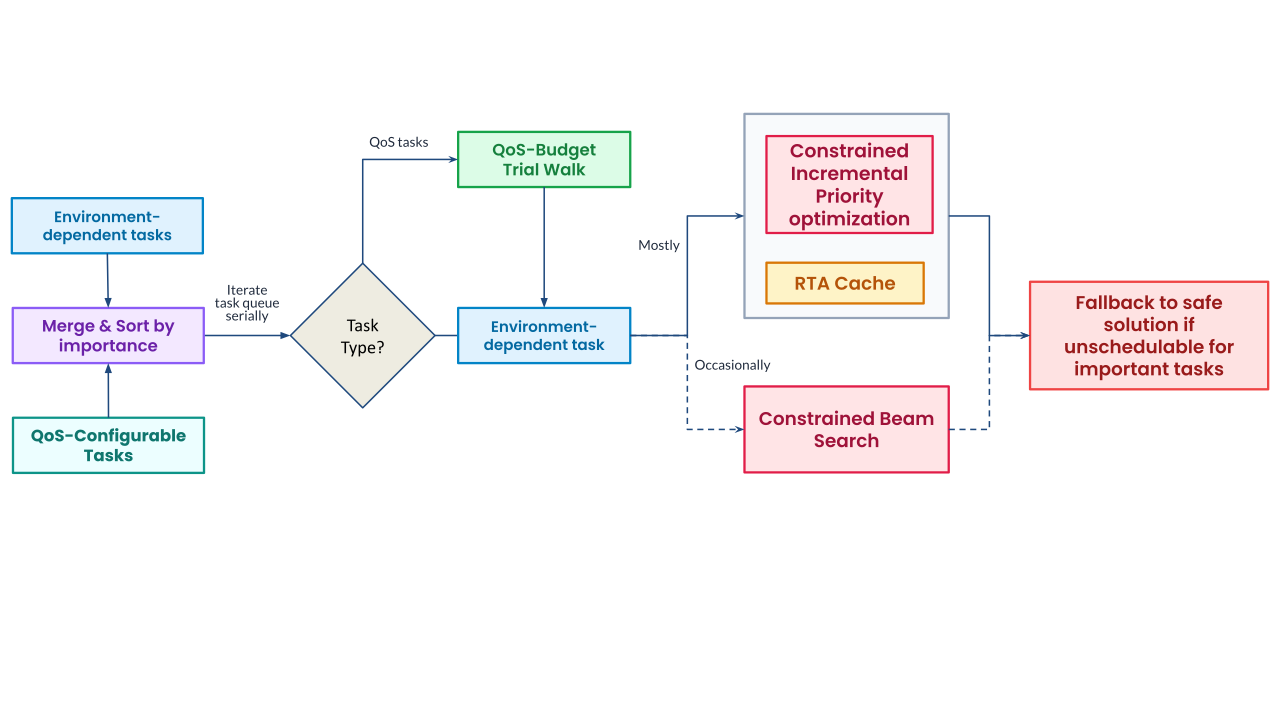
\includegraphics[width=\textwidth]{pictures/overall_workflow.pdf}
        \caption{Overall workflow of the QoS-budget and priority collaborative optimization. 
        The serialized queue sorts environment-dependent ($\tau^E_i$) and QoS-configurable ($\tau^Q_i$) tasks by SP weight $w_i$ descending; 
        each task is dispatched separately to the QoS-budget walk or the incremental priority move, 
        and every accepted single-task adjustment is committed as the champion before the next step, 
        so each evaluation differs from the champion by at most one task and is served from the RTA cache.}
        \label{fig:overall_workflow}
    \end{figure*}

    \subsection{Task Serialization}
    \label{section_task_serialization}

    As introduced in Section~\ref{section: system_model_tasks}, the system has 2 types of tasks: environment-dependent tasks ($\tau^E_i$) whose execution-time distributions are decided by external environment, 
    and QoS-configurable tasks ($\tau^Q_i$) whose execution-time distributions are decided by the internal schedulers.
    To utilize the incremental priority optimization algorithms proposed before, we first sort all the tasks based on their importance and perform optimization to them one by one.

    \subsection{Finding the Initial Solution Before Searching}
    \label{section_initial_solution}

    The compare-and-keep structure of the walk---and the single-change invariant $|\mathrm{diff}|\le 1$ that the RTA cache relies on (Section~\ref{section_rta_cache})---requires a \emph{champion} to exist before the first step: a deployed configuration $\{\boldsymbol{P},\boldsymbol{Q}\}$ together with its SP score and the per-task response-time distributions $\rtDist{i}$ it induces.
    Finding this initial solution is therefore a prerequisite of the search, not a part of it, and it is handled in two regimes that mirror the two descent modes of Section~\ref{section_increment_pa}.

    \textbf{Cold-start seed (interval~0).}
    When the optimizer has no prior incumbent---at the first interval, or whenever a from-scratch re-optimization is triggered with no carried state---it constructs a feasible seed directly rather than searching for one.
    The priority assignment is set by Deadline Monotonic (DM) ordering, $\boldsymbol{P}_{\mathrm{DM}}$, which sorts tasks by deadline ascending; this is preferred over Rate Monotonic because the task set uses constrained deadlines, $D_i = T_i \cdot U(0.5,1.0)$, so the deadline---not the period---is the correct priority key.
    Each QoS-configurable task $\tau^Q_i$ is placed at the smallest budget on its grid, $\boldsymbol{Q}_{\min}$, the option that induces the least interference and is therefore the most likely to be schedulable.
    The pair $\{\boldsymbol{P}_{\mathrm{DM}},\boldsymbol{Q}_{\min}\}$ is scored once under the current execution-time distributions and committed as the champion; the search then proceeds outward from this point.

    \textbf{Warm-started re-score (subsequent intervals).}
    At every later interval the optimizer carries the previous interval's adopted champion forward.
    Because the serialized loop of Section~\ref{section_config_opt} must honor the weight-sorted dispatch order, the carried $\{\boldsymbol{P},\boldsymbol{Q}\}$ is \emph{re-scored} under the interval's drifted execution-time distributions but \emph{not} re-optimized: this is a $|\mathrm{diff}|=0$ full-reuse hit in the RTA cache, so it costs no extra response-time analysis.
    The re-scored value seeds the strict-improvement guard that the walk compares against.

    \textbf{Schedulable seed via the certified fallback.}
    A subtlety of strict-SP compare-and-keep is that it never accepts an SP-lowering move, even one that restores schedulability; a walk that begins from an unschedulable incumbent can therefore terminate on an unschedulable SP-maximal configuration even when schedulable plans of slightly lower SP exist.
    To prevent this, the seed is audited for important-task schedulability at the moment it is scored---again at zero additional RTA cost, since the response-time distributions needed for the constraint $Pr(r_i > D_i) \leq \Theta_i$ of \eqref{eq_important_task_constraint} are exactly those already computed for the SP evaluation.
    If the carried incumbent violates the constraint and a certified safe fallback is available, the fallback's $\{\boldsymbol{P},\boldsymbol{Q}\}$---certified offline against a cross-interval worst-case execution-time distribution that stochastically dominates every interval---is adopted as the seed in its place.
    The walk thus always climbs the SP metric from a schedulable base; the offline construction and adoption contract of this fallback are the subject of Section~\ref{section_safety_fallback}.

    In all regimes the cache is armed \emph{after} the seed is committed: the seed is a $|\mathrm{diff}|=0$ champion, so adopting it is a full-reuse hit, and every subsequent single-task step of the walk satisfies $|\mathrm{diff}|\le 1$ against it.

    \subsection{QoS-Budget Trial-and-Error Walk}
    \label{section_qos_walk}

    For a $\tau^Q_i$ task, the optimizer walks its time-limit grid outward from the current budget, evaluating the SP metric at each option and retaining the best.
    The walk proceeds in two passes from the current option index: first backward (toward smaller budgets), then forward (toward larger budgets).
    A pass halts when it reaches the grid boundary or when a patience budget---a total count of consecutive non-improving steps that is not reset upon an improvement---is exhausted.
    The backward-first ordering serves as a resource-aware tie-break: when two budgets yield equal SP, the smaller one is preferred, conserving computation.
    The patience budget is selected by mode, reflecting that a re-optimization interval (starting from a fresh seed) permits a longer search than an incremental one.

    Each trial budget is evaluated through the incremental priority solver, which re-scores the carried priority assignment together with a single-task priority re-search at the trial budget; because only the walked task's budget differs from the champion, the evaluation is a cache reuse hit.
    Continuing the anytime-algorithm example of Section~\ref{def_task_config}, a motion-planning task with grid $\{100, 200, 300, 500\}$ (in milliseconds) starting from a budget of $300$ tries $200$, then $100$ (the backward pass), then $400$-equivalent options and $500$ (the forward pass), adopting the budget that maximizes the SP metric.

    \subsection{Environment-Task Incremental Priority Move}
    \label{section_env_pa_move}

    For a $\tau^E_i$ task whose distribution changed, the dispatch calls the incremental priority solver of Section~\ref{section_increment_pa} directly---no QoS walk is performed, since the task has no time-limit grid.
    The solver re-searches the task's priority position over one half of the priority range, with the half selected by the four-scenario rule of Section~\ref{section_increment_pa} from the carried change direction, and adopts the best strictly-improving position.
    This is the unification pursued above: both QoS flex and environment change flow through one serialized loop, differing only in the per-task handler, and both reduce to a single-task change that the RTA cache serves incrementally.

    \subsection{Complexity and the Single-Change Property}
    \label{section_complexity_single_change}

    Each pass over the serialized queue evaluates, per $\tau^Q_i$ task, every option it reaches on its grid (bounded by patience) and, per $\tau^E_i$ task, the positions in one half of the priority range; with $N$ tasks in the queue and at most $M$ options per task, the per-pass complexity is $O(M \cdot N)$, a reduction from the $O(M^N)$ exhaustive search over the joint QoS space.
    The full run-time analysis, including the response-time analysis cost folded into each evaluation, is deferred to Section~\ref{section_complexity_analysis}.

    The single-change property is structural: each iteration of the serialized loop adjusts exactly one task's execution-time distribution (via a budget change or an environment change) or priority position, and every accepted adjustment is committed as the new champion before the next iteration begins.
    Consequently every evaluation differs from the champion by at most one task, satisfying the $|\mathrm{diff}| \leq 1$ invariant asserted by the cache's single-change check (Section~\ref{section_rta_cache}); the cache's reuse lemmas therefore apply to every step of the collaborative walk.


	\subsection{RTA Cache: Reusing Response-Time Computation}
	\label{section_rta_cache}

    The incremental optimization needs to repeated analyze the response time distribution of the whole task set, even though the task set is very similar among candidate solutions during the searching process.
    Therefore, following the design that the optimization algorithm iterates through each task one by one, we can design an efficient response time analysis (RTA) cache to significantly speed up RTA.

    In this paper, the rta cache is designed for scenarios where only one task in a task set changes its priority and / or execution time distribution. 
    This is the most frequent scenario during the incremenatl optimization process.
    % This single-change restriction is less severe than it appears, because such candidates are precisely the common case in our framework.
    % The cache holds a \emph{champion}---the current best solution together with the per-task response-time distributions $\rtDist{i}$ it induces---and serves a candidate only when it differs from the champion in at most one task, the \emph{single-change invariant} $|\mathrm{diff}|\le 1$: at most one task $\tau_j$ may change its execution-time distribution $\extDist{j}$, its priority position, or both (a combined change of the same task counts as one); broader changes are rejected and trigger a full recompute.
    % The trigger is frequently satisfied because the incremental optimizer pivots the previous solution one task at a time (Section~\ref{section_increment_pa}), and the PA+QoS loop of Section~\ref{section_config_opt} is structured so that every step changes exactly one task.
    % Consequently the cache applies to nearly every evaluation issued online, converting each $O(N)$-task RTA into a recomputation of only the affected tasks.
% A key property of fixed-priority scheduling is that $\rtDist{k}$ depends only on $\extDist{k}$ and on the execution-time distributions, periods, and \emph{membership} of $\text{hp}(k)$---never on lower-priority tasks or on the order within $\text{hp}(k)$---
% since the RTA~\eqref{eq_prob_rta} builds $\rtDist{k}$ by convolving $\extDist{k}$ with $\{\extDist{\ell}:\tau_\ell\in\text{hp}(k)\}$ and convolution is commutative.
  
    Formally, consider a task set of $n$ tasks, ordered by priority: $\tau_0,\dots,\tau_i,\dots,\tau_j,\dots,\tau_{n-1}$ with $\tau_0$ highest, and let $\text{hp}(k)=\{\tau_0,\dots,\tau_{k-1}\}$.
    Denote the response time of each task $\tau_k$ as $\rtDist{k}$.
    A single-change candidate moves $\tau_j$ up to position $i<j$ (moving $\tau_j$ to a lower priority can be analyzed in a similar way), 
    giving $\tau_0,\dots,\tau_j,\tau_i,\dots,\tau_{n-1}$, and possibly changes $\extDist{j}$.
    Denote the response time distribution of each task after the change as $\rtDisthat{k}$.

    \begin{lemma}[Higher-priority tasks]
    \label{lem:rta_hp}
    For every $k<i$, $\rtDisthat{k}=\rtDist{k}$, regardless of whether $\extDist{j}$ changes.
    \end{lemma}
    \noindent\textit{Proof.}
    In both orderings $\tau_j$ lies below $\tau_k$ (at position $j>k$ before the move, and at position $i>k$ after), so $\tau_j\notin\text{hp}(k)$ in either case and $\text{hp}(k)$ is unchanged. \hfill$\square$

    \begin{lemma}[Lower-priority tasks under a pure priority move]
    \label{lem:rta_lp_pure_move}
    If $\extDist{j}$ is unchanged, then for every $k>j$, $\rtDisthat{k}=\rtDist{k}$.
    \end{lemma}
    \noindent\textit{Proof.}
    $\tau_j\in\text{hp}(k)$ in both orderings and the set $\text{hp}(k)$ is identical; only the order within it is permuted. Since the RTA~\eqref{eq_prob_rta} builds $\rtDist{k}$ by convolving the execution-time distributions in $\text{hp}(k)$, and convolution is commutative, $\rtDisthat{k}=\rtDist{k}$. \hfill$\square$

    \begin{lemma}[Cross-core tasks]
    \label{lem:rta_cross_core}
    For any task $\tau_k$ on a core other than $\tau_j$'s, $\rtDisthat{k}=\rtDist{k}$.
    \end{lemma}
    \noindent\textit{Proof.}
    Under partitioned scheduling, $\tau_j$ never enters $\text{hp}(k)$, so neither its priority move nor its execution-time change affects $\rtDist{k}$. \hfill$\square$
